%%%%%%%%%%%%%%%%%%%%%%%%%%%%%%%%%%%%%%%%%%%%%%%%%%%%%%%%%%%%%%%%%%%%%%%%%%%%
%
% FILE      : legoman.tex
% Time-stamp: <2004-09-13 14:18:52 ssardina>
%
%       LeGolog manual
%
%  Author : Sebastian Sardina
%  email  : ssardina@cs.toronto.edu
%  WWW    : www.cs.toronto.edu/~ssardina www.cs.toronto.edu/cogrobo
%  TYPE   : manual 
%
%%%%%%%%%%%%%%%%%%%%%%%%%%%%%%%%%%%%%%%%%%%%%%%%%%%%%%%%%%%%%%%%%%%%%%%%%%%%
\documentclass[11pt]{article}

%%%%%%%%%%%%%%%%%%%%%%%%%%%%%%%%%%%%%%%%%%%%%%%%%%%%%%%
% PACKAGES TO LOAD
%%%%%%%%%%%%%%%%%%%%%%%%%%%%%%%%%%%%%%%%%%%%%%%%%%%%%%%
% Loading of Babel language library
%\usepackage[spanish,english]{babel}
%\usepackage[asciiext]{inputenc}

% Loading of symbols libraries
\usepackage{fullpage}     % To get full-page documments
\usepackage{amsmath}
\usepackage{latexsym}
\usepackage{amssymb}
\usepackage{psfrag}       % Replace utility in pictures
\usepackage{graphicx}     % \includegraphics[]{}
\usepackage[active]{srcltx}

\usepackage{color}
\definecolor{darkgreen}{rgb}{0,0.6,0}
\usepackage[ps2pdf=true,
 letterpaper=true,
 pagebackref=true,
 hyperindex=true,
 colorlinks=true,
 linkcolor={blue},
 citecolor={darkgreen},
 pdftitle={Title...},
 pdfauthor={Author...},
 pdfsubject={Subject...},
 pdfkeywords={Keywords...},
 pdfhighlight={/O}]{hyperref}

%%%%%%%%%%%%%%%%%%%%%%%%%%%%%%%%%%%%%%%%%%%%%%%%%%%%%%%
% TITLE INFORMATION AND MARGIN DESIGNS
%%%%%%%%%%%%%%%%%%%%%%%%%%%%%%%%%%%%%%%%%%%%%%%%%%%%%%%
\title{
\vfill 
{\huge \PIndiGolog: An Integrated Agent Architecture} \\
\vfill
{\Large Programmer and User Manual \\
Beta Version 0.3} \\
\vfill
}
\author{Sebastian Sardi\~na}


%%%%%%%%%%%%%%%%%%%%%%%%%%%%%%%%%%%%%%%%%%%%%%%%%%%%%%%%%%%%%%%%%%%%%%%%%%%%
%%%%%%%%%%%%%%%%%%%%%%   User defined macros - START %%%%%%%%%%%%%%%%%%%%%%%
%%%%%%%%%%%%%%%%%%%%%%%%%%%%%%%%%%%%%%%%%%%%%%%%%%%%%%%%%%%%%%%%%%%%%%%%%%%%

%%% Knowledge 
\newcommand{\Know}{\mbox{\bf Know}}
\newcommand{\KWhether}{\mbox{\bf KWhether}}
\newcommand{\KHow}{{\bf KnowHow}}
\newcommand{\Kref}{\mbox{\bf KRef}}


%%% Ability
\newcommand{\Achieve}{\mbox{\bf Achieve}}
\newcommand{\Can}{\mbox{\bf Can}}
\newcommand{\CanFollow}{\mbox{\bf CanFollow}}
\newcommand{\CanGet}{\mbox{\bf CanGet}}
\newcommand{\OnPath}{\mbox{\bf OnPath}}
\newcommand{\CanBot}{\mbox{\bf Can}_{\perp}}
\newcommand{\CanIterK}{\mbox{\bf Can}^{k}_{I}}

\newcommand{\Goal}{\mbox{\bf Goal}}
\newcommand{\OGoal}{\mbox{\bf OGoal}}
%\newcommand{\Domin}{\mbox{\bf Dominates}}
\newcommand{\Domin}{\mbox{\bf Dom}}
\newcommand{\Rational}{\mbox{\bf Rational}}
\newcommand{\RationalPrio}{\mbox{\bf RationalPrio}}


%% Programs
\newcommand{\mif}{\mbox{\bf if}}
\newcommand{\mwhile}{\mbox{\bf while}}
\newcommand{\mreturn}{\mbox{\bf return}}
\newcommand{\mthen}{\mbox{\bf then}}
\newcommand{\melse}{\mbox{\bf else}}
\newcommand{\mdo}{\mbox{\bf do}}
\newcommand{\mnoOp}{\mbox{\bf noOp}}
\newcommand{\mproc}{\mbox{\bf proc}}
\newcommand{\mend}{\mbox{\bf end}}
\newcommand{\mendproc}{\mbox{\bf endProc}}
\newcommand{\mendif}{\mbox{\bf endIf}}
\newcommand{\mendwhile}{\mbox{\bf endWhile}}
\newcommand{\mendfor}{\mbox{\bf endFor}}
\newcommand{\mfor}{\mbox{\bf for}}
\def\prparallel{\mathrel{\rangle\!\rangle}}
\def\supparallel{\mathord{|\!|}}
\newcommand{\search}{\mbox{$\Sigma$}}
\newcommand{\searchE}{\mbox{$\Delta_e$}}
\newcommand{\searchM}{\mbox{$\Delta_{em}$}}
\newcommand{\searchL}{\mbox{$\Delta_l$}}
\newcommand{\mnt}{\mbox{$mnt$}}

% Caligraphic letters
\newcommand{\DD}{\mbox{$\cal D$}}                     % Calligraphic D
\newcommand{\TT}{\mbox{$\cal T$}}                     % Calligraphic T
\newcommand{\CC}{\mbox{$\cal C$}}                     % Calligraphic C

%%%%% Formulas
\newcommand{\isdef}{\hbox{$\stackrel{\mbox{\scriptsize\rm def}}{=}$}}
\newcommand{\isdeff}{\: \isdef \:}
\newcommand{\Eventually}{\mbox{\bf Eventually}}
\newcommand{\Always}{\mbox{\bf Always}}

% Others (tools...)
\newcommand{\comment}[1]{}
\newcommand{\finishpage}{ \newpage{ \pagestyle{empty} } }



%%%%%  Extra macros

\gdef\M#1{\ifmmode #1\else$#1$\fi}
\newcommand{\now}{{\hbox{\small\sf now}}}
\newcommand{\start}{{\hbox{\small\sf start}}}
\newcommand{\psend}{{\hbox{\small\sf end}}}
\newcommand{\disp}[1]{\[#1\]}
\newcommand{\wff}[1]{{\M{#1}}}
\newcommand{\sit}[1]{{\M{#1}}}
\newcommand{\var}[1]{{\M{#1}}}
\newcommand{\constant}[1]{{\M{#1}}}
\newcommand{\act}[1]{{\M{#1}}}
\newcommand{\inisit}{\sit{S_0}}
\newcommand{\Do}{{\M{Do}}}
\newcommand{\sdo}{{\M{do}}}
\newcommand{\Poss}{{\M{Poss}}}

\newcommand{\Done}{\mbox{\bf Done}}
\newcommand{\geqsig}{\succeq}
\newenvironment{eqns}{\protect\[\begin{array}{l}}{\end{array}\protect\]}

\newcommand{\ind}{\hspace{1em}}
\newcommand{\nowsig}{{\hbox{\small\sf asf}}}
\newcommand{\nowsit}{{\hbox{\small\sf sit}}}

\newcommand{\nlf}{\sc}                   % font for non-logical symbols
\newcommand{\nonlg}[1]{\mbox{\nlf #1}}


\newcommand{\LeGolog}{\mbox{\textsc{LeGolog}}}
\newcommand{\PIndiGolog}{\mbox{\textsc{P-IndiGolog}}}
\newcommand{\IndiGolog}{\mbox{\textsc{IndiGolog}}}
\newcommand{\Golog}{\mbox{\textsc{Golog}}}
\newcommand{\ConGolog}{\mbox{\textsc{ConGolog}}}
\newcommand{\Prolog}{\mbox{\textsc{Prolog}}}


%%%%%%%%%%%%%%%%%%%%%%%%%%%%%%%%%%%%%%%%%%%%%%%%%%%%%%%%%%%%%%%%%%%%%%%%%%%%
%%%%%%%%%%%%%%%%%%%%%%   User defined macros - END %%%%%%%%%%%%%%%%%%%%%%%%%
%%%%%%%%%%%%%%%%%%%%%%%%%%%%%%%%%%%%%%%%%%%%%%%%%%%%%%%%%%%%%%%%%%%%%%%%%%%%


%%%%%%%%%%%%%%%%%%%%%%%%%%%%%%%%%%%%%%%%%%%%%%%%%%%%%%%%%%%%%%%%%%%%%%%%%%%%
%%%%%%%%%%%%%%%%%%%%%%   Environments - START  %%%%%%%%%%%%%%%%%%%%%%%%%%%%%
%%%%%%%%%%%%%%%%%%%%%%%%%%%%%%%%%%%%%%%%%%%%%%%%%%%%%%%%%%%%%%%%%%%%%%%%%%%%
\newtheorem{subtheorem}{Theorem}[subsection]
\newtheorem{theorem}{Theorem}[section]
\newtheorem{conjecture}[theorem]{Conjecture}
\newtheorem{corollary}[theorem]{Corollary}
\newtheorem{definition}[theorem]{Definition}
\newtheorem{proposition}[theorem]{Proposition}
\newtheorem{lemma}[theorem]{Lemma}
\newtheorem{example}[theorem]{Example}

\newcommand{\Theorem}[1]{ \begin{theorem} #1 \end{theorem} }
\newcommand{\Definition}[1]{ \begin{definition} #1 \end{definition} }
\newcommand{\Lemma}[1]{ \begin{lemma} #1 \end{lemma} }
\newcommand{\Claim}[1]{ \begin{claim} #1 \end{claim} }
\newcommand{\Example}[1]{ \begin{example} #1 \end{example} }

%%%%%%%%%%%%%%%%%%%%%%%%%%%%%%%%%%%%%%%%%%%%%%%%%%%%%%%%%%%%%%%%%%%%%%%%%%%%
%%%%%%%%%%%%%%%%%%%%%%   Environments - END  %%%%%%%%%%%%%%%%%%%%%%%%%%%%%%%
%%%%%%%%%%%%%%%%%%%%%%%%%%%%%%%%%%%%%%%%%%%%%%%%%%%%%%%%%%%%%%%%%%%%%%%%%%%%





% ============================================================================
% =======================BEGINNING OF THE DOCUMENT============================
% ============================================================================
\begin{document}

\maketitle                % Title Generation
\pagebreak
\tableofcontents        % Index Generation
\pagebreak
%\thispagestyle{empty}   % No numbering for this title page

%%%%%%%%%%%%%%%%%%%%%%%%%%%%%%%%%%%%%%%%%%%%%%%%%%%%%%%%%%%%%%%%%%%%%%%%%%%%
\section{OVERVIEW}

\PIndiGolog\ \cite{Levesque00-Legolog} is an agent architecture completely
programmed in \Prolog\ which intends to realize the \IndiGolog\ logic-based
interleaved agent account of sensing, planning, and
execution \cite{Giuseppe99-IncremInt,Sardina00MSc,Lesperance00,
Giuseppe01,Giuseppe02, SardinaPhd05}. 
%
\PIndiGolog\ is based on \LeGolog\\cite{Levesque00-Legolog}, a logic-programming
architecture for running \Golog\ \cite{Levesque97-Golog} agent programs on the
LEGO MINDSTORMS Robotic Invention System (RIS).\footnote{See
\texttt{http://mindstorms.lego.com} and
\texttt{http://www.cs.toronto.edu/cogrobo/Legolog/index.html}}
%
\PIndiGolog, however, can be used with any real robotic or virtual platform,
provided the correct device managers are written. At this point, we have used
\PIndiGolog\ to control the LEGO MINDSTORM robot already mentioned as well as
the ER1 EVOLUTION robot\footnote{See \texttt{http://www.evolution.com/}} and
several Internet and System agents. We plan to use it to control the RWI R21
robot too.\footnote{See
  \texttt{http://www.irobot.com/rwi/p06.asp}}

This manuscript is intended to give a quick overview of the \PIndiGolog\
architecture \textit{internal implementation}. Thus, it is mainly aimed for the
programmer/developer of the architecture. Nevertheless, the regular user may
just jump directly to Section \ref{sec:user} in order to find instructions and
guidelines on how to develop domain applications for the \PIndiGolog\ agent
system. 


A quick graphical overview of the complete architecture is shown in Figure
\ref{FigLeGolog}. The outline of this manual is as follows: 
%
\begin{description}
\item[Section \ref{sec:dirstruct}:] Describes the logical directory structure of
\PIndiGolog. The architecture is modular divided into many files and each file
is placed in a particular directory depending on its role within the framework.

\item[Section \ref{sec:main}:] Discusses the core of the architecture, namely,
the main top-level control cycle and the module in charge of communicating with
the external devices and environments.\footnote{From now on, the external,
real-world, systems that will interact with \PIndiGolog\ will be refer to
devices (e.g., a real robotic platform) or environments (e.g., the Internet, a
file system).} 

\item[Section \ref{sec:eval}:] Discusses the role of the evaluation procedure
or temporal projector.

\item[Section \ref{sec:environments}:] Outlines the form and interface of the
device managers, which are the modules in charge of managing each external
device or environment (e.g., a robot platform). After reading this section, the
reader should be able to design new device managers to operate new robots or
environments.

\item[Section \ref{sec:user}:] Provides detailed guidelines on how to
use \PIndiGolog\ for a real domain application. This section amounts to
the ``User Manual'' and should be sufficient for anybody wanting to use
\PIndiGolog.

\item[Section \ref{sec:todo}:] Discusses future improvements.

\item[Section \ref{sec:links}:] Lists related pointers and references.

\item[Section \ref{sec:conclusions}] Draws conclusions.
\end{description}


\begin{figure*}[b]
\begin{center}
%\psfrag{K}{$K$}
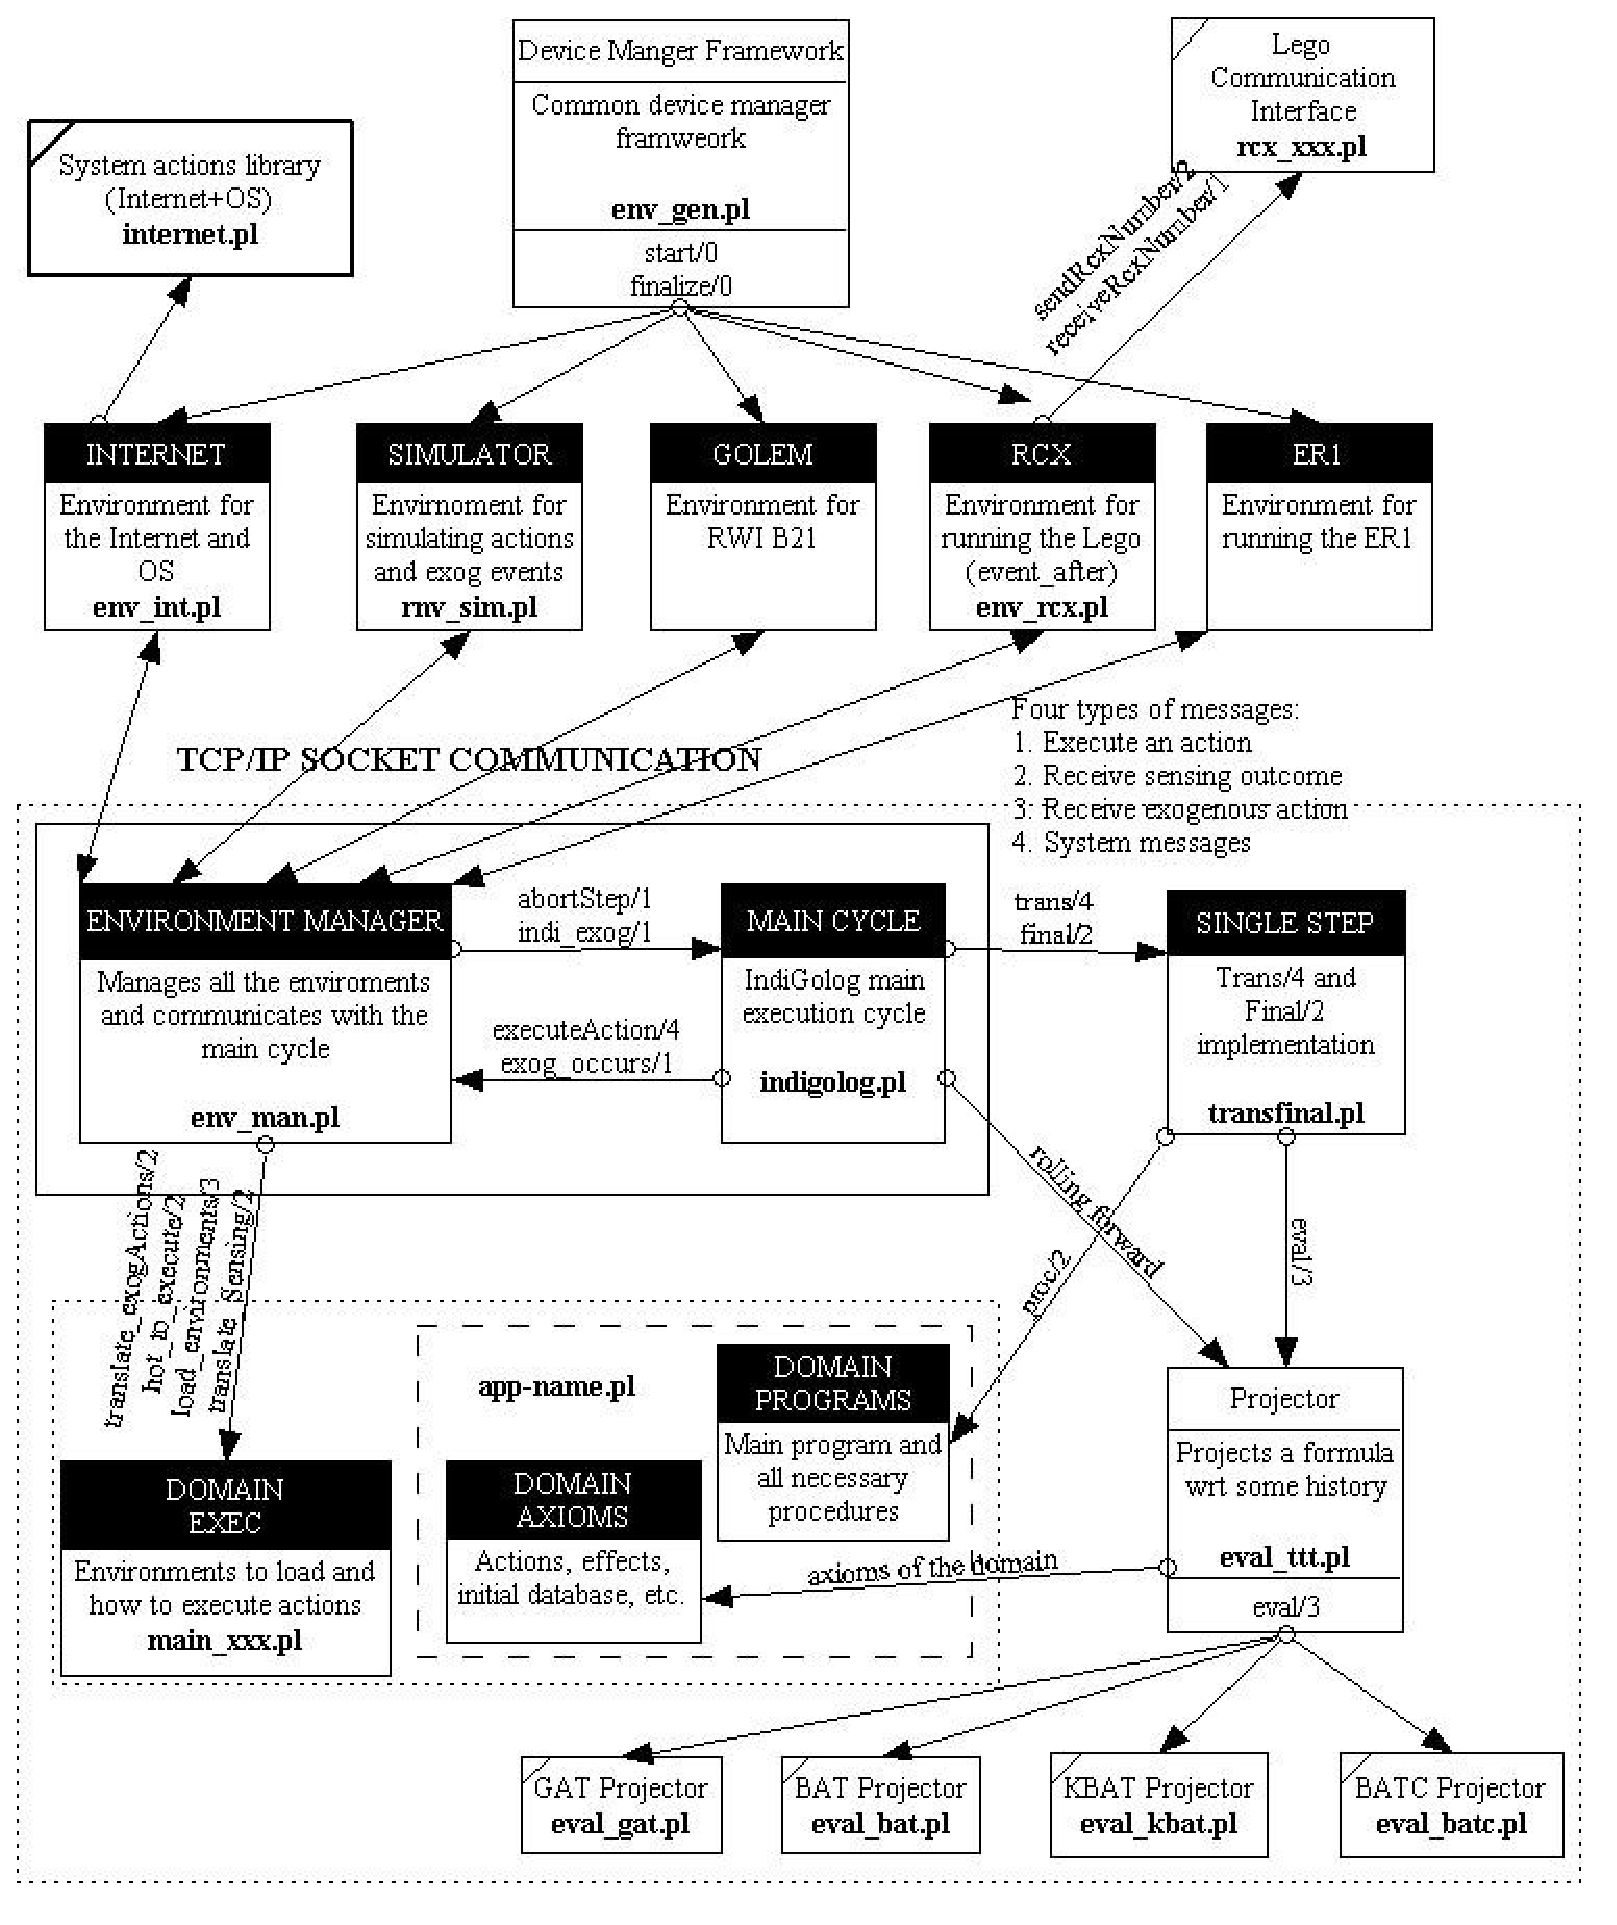
\includegraphics[height=17cm,width=17cm]{system.eps}
\caption{The \PIndiGolog\ architecture}
\label{FigLeGolog}
\end{center}
\end{figure*}

% We point out that this document is not intended to be the ``programmer''
% documentation as most of the low-level programming details will be completely
% ignored. The objective, instead, is to easily introduce the reader to the
% \PIndiGolog\ framework by showing the main role of each module, the
% interaction
% among them, and their most important predicates. The reader should consult the
% internal documentation for implementation details.


%%%%%%%%%%%%%%%%%%%%%%%%%%%%%%%%%%%%%%%%%%%%%%%%%%%%%%%%%%%%%%%%%%%%%%%%%%%%%%%%
\section{DIRECTORY LOGICAL STRUCTURE} \label{sec:dirstruct}

The files conforming the whole implementation are scattered among many different
directories. Knowing the logical structure facilitates the task of finding files
and locating specific code depending on its nature.
%
In order to use \PIndiGolog, the global environment variable
\texttt{PATH\_INDIGOLOG} must point to the architecture root directory (e.g., 
\texttt{PATH\_INDIGOLOG=/home/ssardina/Code/indigolog}).
Environment variable \texttt{PATH\_INDIGOLOG} is often used to localize
libraries and specific files. From the architecture initial directory, the
logical directory structure is as follows:

\begin{description}
\item[\texttt{Doc/}] Documentation, manuals, guides, logos, etc. For instance,
this manual is inside this directory.
  
\item[\texttt{Env/}] All code related to the handling of the external
environments. All device managers (see Section \ref{sec:environments}) and the
environment manager itself (see Section \ref{sec:envmanager}) are located in
this directory.
  
\item[\texttt{Eval/}] Temporal projectors or evaluation procedures (see Section
  \ref{sec:eval}).
  
\item[\texttt{Interpreters/}] Top-level architecture module (see Section
  \ref{sec:maincycle}) and the any transition system available.

\item[\texttt{Lib/}] Compatibility and tool libraries, global definitions.

  
\item[\texttt{Examples/}] Domain applications (e.g., elevator controller,
  delivery coffee robot, etc.). For legibility and modularity, each application
should be stored in its own subdirectory (Section \ref{sec:user}).
  
\item[\texttt{Old/}] Old code that is out of use but that we may want to keep.

\item[\texttt{Temp/}] Temporal directory.
\end{description}




\subsection{Libraries Provided}

Among others, these are some of the libraries provided in directory
\texttt{Lib/}:
\begin{itemize}
\item \texttt{eclipse\_swi.pl}: SWI library for compatibility with ECLIPSE
\Prolog.

\item \texttt{common.pl}: \Prolog\ independent common library.

\item \texttt{tools\_xxx.pl}: tool library for \Prolog\ \texttt{xxx}. Currently,
we have special libraries for ECLIPSE \Prolog\ (\texttt{tools\_ecl.pl}) and
SWI \Prolog\ (\texttt{tools\_swi.pl}). These libraries usually include library
\texttt{common.pl}


\item \texttt{systemvar.pl}: library used by domain applications' main
files to perform \Prolog\ initializations.

\item \texttt{er1actions.pl}: library for translating ER1 actions to their
low-level representations.
\end{itemize} 



%%%%%%%%%%%%%%%%%%%%%%%%%%%%%%%%%%%%%%%%%%%%%%%%%%%%%%%%%%%%%%%%%%%%%%%%%%%%
\section{THE CORE \label{sec:main}}

The core of the \PIndiGolog\ is made of two modules, namely, the top-level
\emph{main cycle} and the \emph{environment manager}.
%
The former implements the main loop of the system which is based on the
well-known \textit{sense-think-act} loop in the agent community
\cite{Kowalski95}.
%
The latter module provides the interfaces with the external world, which is
viewed as a set of different devices and environments. 
%
So, for example, whenever the main cycle produces an action to be executed, it
passes the action to the environment manager which, in turn, will communicate
with the corresponding device in order to execute the action in question.
Similarly, whenever a device or environment produces an exogenous event, this
is passed to the environment manager which, in turn, will pass it to the main
cycle as it corresponds.


%%%%%%%%%%%%%%%%%%%%%%%%%%%%%%%%%%%%%%%%%%%%%%%%%%%%%%%%%%%%%%%
\subsection{The Top-Level Main Cycle \label{sec:maincycle} }

The \textit{top-level main cycle} is intended to execute a
\textit{sense-think-act} interleaved loop in the spirit of many state of the art
agent systems \cite{Kowalski95}. In a nutshell the cycle repeats the following
four steps continuously: (i) roll forward the database if necessary; (ii)
check for exogenous events that have occurred; (iii) calculate the next program
step; and (iv) if the step involves an action, execute the action.

The execution of an agent program \texttt{E} is started in \PIndiGolog\ by
calling predicate \texttt{indigolog(E)}. First, \texttt{init/0} is called to
perform some system-wide initializations. Then, the top-level \textit{main
cycle} is started by calling \texttt{indigo/2} with the main program and the
empty history. When the cycle terminates, \texttt{fin/0} is called to perform
system-wide finalization routines.

So, \texttt{indigo/2} implements the top-level cycle. It be found in file
\texttt{Interpreters/indigolog.pl} and is depicted in Figure
\ref{fig:legocycle}. Roughly speaking, the cycle can be described
as follows:

\renewcommand{\labelenumii}{\arabic{enumi}.\arabic{enumii}.}
\renewcommand{\labelenumiii}{\arabic{enumi}.\arabic{enumii}.\arabic{enumiii}.}

\begin{enumerate}
\item Perform \textbf{mandatory rolling forward} of the database by
calling \texttt{handle\_rolling/2} (e.g., whenever the history has grown
excessively long).

\item Handle all pending \textbf{exogenous events} by calling
\texttt{handle\_exog/2}.
  
\item Compute the next \textbf{legal transition step} by calling
\texttt{mayEvolve/5}, which, in turn, uses the underlying transition system.
Depending on the outcome of this step, the cycle proceeds as follows:

\begin{enumerate}
\item If the step was \textbf{interrupted} by an exogenous event before
termination, then abort step and jump to step (1) without changing the current
configuration (i.e., the program and history).
    
\item If the current configuration was found to be \textbf{final}, then
\emph{terminate successfully} the top-level cycle. At this point,
\texttt{indigo/2} just succeeds.
       
\item If a \textbf{legal transition step} was indeed found, then do the
following in priority order:
%
\begin{enumerate}
\item If the step found \textit{does not involve a new action} (i.e., the
history remains the same), then restart the cycle in (1) with the new remaining
program but the same history.
         
\item If the step found involves a \emph{simulated} action (i.e., action
of the form \texttt{sim(A)} for some real action \texttt{A}), then ignore the
action and restart the cycle in (1) with the new remaining program but the same
history.
      
\item If the step found is the \emph{waiting} meta-action \texttt{wait}, then
perform optional rolling forward and, then, wait for an exogenous action to
occur by using predicate \texttt{doWaitForExog/2}. After an exogenous event
happen, restart the cycle in (1) without including the action \texttt{wait}.
      
\item If the step found is a \texttt{show\_debug} action, then start
debugging by calling \texttt{debug/3} projector tool. When finished,
restart cycle in (1) without including the \texttt{show\_debug} action.
    
\item If the step involves a \texttt{halt\_exec} action, then restart the
cycle in (1) with the empty program.

\item If the step involves an \texttt{abort\_exec} action, then restart the
cycle in (1) with the always failing program \texttt{?(false)}.

\item If the step involves an \texttt{pause\_exec} action, then a
\Prolog\ break point is inserted to the main cycle. It is not possible to
use the \Prolog\ prompt to perform queries (for debugging mainly) and restart
the program execution by just typing \texttt{Ctrl+D}.

\item If the step found is a \texttt{stop\_interrupts} action, then just restart
the cycle in (1).
         
\item Finally, if the step found involves a particular \textit{domain
action}, then execute the action in question in the real world by calling
\texttt{indixeq/3} and, after that, restart the cycle in (1) with the remaining
program and the new updated history.
\end{enumerate}
\end{enumerate}
\end{enumerate}


The main cycle makes use of the following auxiliary tools:

\begin{itemize}
\item \texttt{now(-H)}: \texttt{H} is the current history in the system. All
the actions in \texttt{H} have already been executed.

\item \texttt{indi\_exog(-A)}: \texttt{A} is an exogenous action that has
occurred
  but has not yet been handled, i.e., has not been incorporated into the
  current history.
\item \texttt{doingStep/0}: states whether a next-step-transition is being
  computed.
\end{itemize}

Predicate \texttt{indigo/2} uses several important tools:

\begin{itemize}
\item \texttt{handle\_rolling(+H, -H2)}: implements the \emph{mandatory} rolling
forward of history \texttt{H} to history \texttt{H2}. The history must be 
rolled  forward in certain circumstances (e.g., the history has grown up to
long). The predicate uses \texttt{must\_roll/1} and \texttt{roll\_db/2}
from the temporal projector (Section \ref{sec:eval}).
  
\item \texttt{pause\_or\_roll(+H, -H2)}: implements the \emph{optional} rolling
forward of current history \texttt{H} to history \texttt{H2}. In this case,
the history should be roll forward if there is sufficient time to do so. 
The predicate uses \texttt{can\_roll/1} and \texttt{roll\_db/2}
from the temporal projector (Section \ref{sec:eval}).
  
\item \texttt{handle\_exog(+H, -H2)}: handles the pending exogenous actions
which are stored under clause \texttt{indi\_exog/1}. Basically, this amounts to
adding all pending exogenous actions into the current history defined by
\texttt{now/1}.
  
\item \texttt{indixeq(+A, +H, -S)}: execute domain action \texttt{A} at history
  \texttt{H} in the real world with sensing outcome value \texttt{S}.  The
  predicate interacts with the \emph{environment manager} via predicate
  \texttt{execute\_action/4}, which will order the execution of the
  action in the corresponding device manager.
  %
  If the sensing outcome is bound to term \texttt{failed}, then
  \texttt{action\_failed/2} is called. Otherwise, \texttt{indixeq/3} updates the
  \texttt{now/1} predicate by  appending action \texttt{A} to the current system
  history.
  
\item \texttt{mayEvolve(+E1,+H1,-E2,-H2,-S)}: this may be the most
  important predicate as it defines the transition between one state of the
  system and the next one. 
  %
  In a nutshell, it says to system configuration \texttt{(E1,H1)} can
  evolve to configuration \texttt{(E2,H2)} under step type \texttt{S}.
  If a legal step could be found (i.e., \texttt{S=trans}), \texttt{E2} would
  stand for the remaining program and \texttt{H2} for the new history.

  \begin{description}
  \item[\texttt{S=trans}] configuration \texttt{(E1,H1)} can legally advance one
    step to configuration \texttt{(E2,H2)} w.r.t. the underlying transition
    system.
    
  \item[\texttt{S=final}] configuration \texttt{(E1,H1)} can legally terminate
  successfully w.r.t. the underlying transition system. Variables \texttt{E2}
and
  \texttt{H2} have no meaning here.
    
  \item[\texttt{S=exog}] an exogenous event occurred during the computation of
    \texttt{mayEvolve/5}. So far, variables \texttt{E2} and \texttt{H2} have no
    meaning in this case. However, in the future, these variables may be used
    as partial information regarding the computation performed by
    \texttt{mayEvolve/5} up to the point of interruption.
    
  \item[\texttt{S=failed}] the current configuration \texttt{(E1,H1)} cannot
    terminate and cannot make any legal transition w.r.t. the underlying
    transition system. In this case, the  configuration has reached a so-called
    dead-end and the program is ``stuck''.
    Variables \texttt{E2} and \texttt{H2} have no meaning in this case.
  \end{description}
  
  As expected, predicate \texttt{mayEvolve/5} depends on an underlying
  transition system. Such transition system should be defined by two
  predicates: \texttt{trans/4} and \texttt{final/2}, which are implemented in
  file \texttt{Interpreters/transfinal.pl} and have the following
  interpretation:
  \begin{itemize}
  \item \texttt{trans(+E1,+H1,-E2,-H2)} succeeds if there is a legal transition
    from configuration \texttt{(E1,H1)} to configuration \texttt{(E2,H2)}.
    
  \item \texttt{final(+E,H)} succeeds if \texttt{(E,H)} is a terminating
    configuration.
  \end{itemize}

\item \texttt{indigo2/2}: implements the \textit{second} phase of the main cycle
whenever a transition was found. If the transition found involves no new action,
then \texttt{indigo/2} is called directly with the new program. 
However, if the transition involves a new action, then there are two general
cases. If the action in question is a \textit{system} action (i.e., an action
that is not intended to be performed by our agent, but one that carries some
special meaning in the top-level loop), then some particular task is performed
and the main cycle is restarted by calling \texttt{indigo/2}. At the moment, the
following are considered system actions:
%
\begin{itemize}
\item \underline{Simulated actions}: this is an action of the form
\texttt{sim(\_)} and it means that the action was just used for simulation and
it should not be actually performed. Hence, it the step is just ignored and the
\texttt{indigo/2} is called.

\item \underline{Wait for an exogenous action}: this is an action called
\texttt{wait} and it sets the system to just wait until some exogenous action
happens. Then, the main cycle is restarted.

\item \underline{Call for debugging}: this is an action called
\texttt{show\_debug}. The debugging predicate \texttt{debug/3} is called and the
main cycle restarted.

\item \underline{Halt/Abort system}: this are meta-actions called
\texttt{halt\_exec} and \texttt{abort\_exec}, respectively, that causes the
system to terminate abruptly either successfully or by failing completely.

\item \underline{Pause system}: this is a meta-actions called
\texttt{pause\_exec} that causes the top-level cycle to pause by introducing a
\Prolog\ \texttt{break} point. It is possible then to perform queries using the
\Prolog\ top-level prompt and return to the program execution by doing
\texttt{Ctrl+D}.


\item \underline{Stop interrupts}: this is an action called
\texttt{stop\_interrupts} and it is used to stop the handling of high-level
interrupts.
\end{itemize} 

If the action corresponding to the transition is \textit{not} one of the above
system actions, then it ought to be a domain specific action, i.e., one that
the agent/robot should perform in the real world. As a result, the action is
sent for real execution using predicate \texttt{indixeq/3} and the main cycle
is restarted after that.
    
\item \texttt{abortStep/0}: this predicate is called when the main cycle is in
  the process of computing an system evolution step (i.e., \texttt{mayEvolve/5}
  is  executing) and an exogenous event arrives asynchronously. 
  The predicate is generally coupled with the implementation for
  \texttt{mayEvolve/5} by appealing to event handling mechanisms in order to
  interrupt the execution of a \Prolog\ goal.
  For example, \texttt{abortStep/0} may throw an exception that
  \texttt{mayEvolve/5} can recognize and act upon.
\end{itemize}




\begin{figure}
\begin{center}
\psfrag{mrolling}{Mandatory rolling forward}
\psfrag{exogevents}{Handle exogenous events}
\psfrag{step}{Calculate next step}
\psfrag{end}{Computation terminated!}
\psfrag{interrupted}{\parbox{2cm}{Exog. \\ event \\ occurred!}}
\psfrag{exogevents}{Handle exogenous events}
\psfrag{wait}{\parbox{2cm}{Wait for \\ exog. event}}
\psfrag{exec}{\parbox{2cm}{Execute \\ action}}
\psfrag{newstep}{\parbox{2cm}{Type \\ of \\ step?}}
\psfrag{voidstep}{test/simulated action}
\psfrag{domstep}{\parbox{2cm}{domain \\ action}}
\psfrag{waitstep}{wait action}
\psfrag{final}{\small final}
\psfrag{trans}{\small trans}
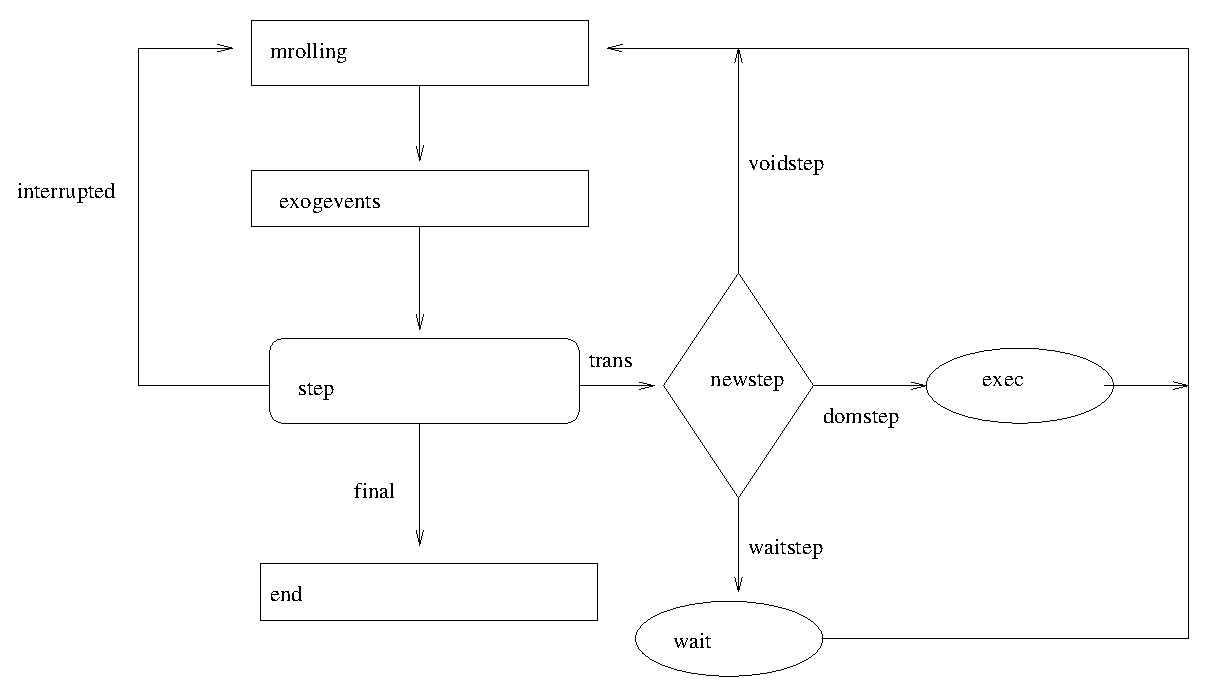
\includegraphics[width=17cm]{legocycle.eps}
\caption{The \PIndiGolog\ top-level cycle}
\label{fig:legocycle}
\end{center}
\end{figure}


%%%%%%%%%%%%%%%%%%%%%%%%%%%%%%%%%%%%%%%%%%%%%%%%%%%%%%%%%%%%%%%
\subsection{EM: The Environment Manager \label{sec:envmanager}}

The environment manager (EM) is tightly coupled with the main cycle and
provides a complete interface with all the external devices, platforms, and
real-world environments.
%
In a nutshell, the EM is responsible of executing actions in the real world and
gathering information from it in the form of sensing outcome and exogenous
events.
%
The full EM implementation can be found at \texttt{Env/env\_man.pl}

Given a domain high-level action, the EM is in charge of: (i) deciding which
device should execute the action; (ii) order its execution to the appropriate
device manager; and (iii) collect the corresponding sensing outcome.  
%
Furthermore, the EM is continuously listening to the devices for the
occurrence of exogenous events.

When the system starts, the EM starts up all device managers required by the
application and sets up communications channels to them using TCP/IP stream
sockets. Recall that each real world device or environment has to have a
corresponding device manager that understands it.
%
After this initialization process, the EM enters into a \textit{passive mode}
in which it asynchronously listens for messages arriving from the various
devices managers. This passive mode should allow the top-level main cycle to
execute without interruption until a message arrives from some device manager.
%
In general, a message can be an exogenous event, a sensing outcome of some
recently executed action, or a system message (e.g., a device being
closed unexpectedly).  The incoming message should be read and handled in an
appropriate way, and, in some cases, the top-level main cycle should be
notified of the occurred event.

Three different implementations are provided via \texttt{env\_man\_cycle/1} for
realizing this passive mode. The first implementation is based on \emph{software
signals} or interrupts; the second one is based on systematic
\textit{after-events}; and the the third one is based on \emph{multi-threading}.
Whereas the third one works on BSD systems only (e.g., Unix, Linux, etc),
the second one works with \Prolog\ implementations supporting after-events
(e.g., ECLIPSE \Prolog), and the first one works only on multi-threading
\Prolog\ implementations (e.g., SWI-\Prolog). More details on these
implementations are described below.

%%%%%%%%%%%%%%%%%%%%%%%%%%%%%%%%
\subsubsection{The EM Interface}

We now list and explain the predicates which conform the EM interface to 
the main top-level cycle of the architecture.

\begin{itemize}
\item \texttt{initializeEM/0}: this predicate is called just once to start the
EM. Generally, this is done at the very beginning of the architecture
initialization. Basically, it performs the following two steps:
\begin{enumerate}
\item Initializes all the device managers required for running the
    application using \texttt{start\_env/2}. The domain application specifies
    which devices are required to load by using predicate
    \texttt{load\_environment/3} (see Section \ref{sec:user}).
    %
    This process involves, among other things, establishing a socket
    connection with each device manager in order to be able to communicate
    with them during the complete execution.
    
 \item Starts the EM passive-mode cycle using \texttt{start\_env\_cycle/1} 
depending on they kind of implementation chosen: \textit{threads},
\textit{after-events}, or \textit{signals/interrupts}. The passive mode cycle is
responsible of watching, passively, the 
  connections to the various device managers for asynchronous messages
  (e.g., exogenous events, sensing outcomes, and system messages). This task
  should be programmed in such a  way that an asynchronous event coming from any
  device manager could eventually interrupt the top-level execution if
  required. 
  More information on how this cycle is implemented is given in the following
  section.
\end{enumerate}
  
  
\item \texttt{finalizeEM/0}: this predicate is the counterpart of
\texttt{initializeEM/0} and is called when the application has completely
finished. The predicate performs the following sequence of actions:
\begin{enumerate}
  \item Closes all open device managers by calling \texttt{close\_dev/1}, which,
  in turn, sends each device a specific ``closing'' message.

\item Terminates the EM passive-mode cycle using \texttt{finish\_env\_cycle/1}. 
\end{enumerate}
  
\item \texttt{execute\_action(+A, +H, +T, -S)}: this predicate is called by the
top-level main cycle whenever an action needs to be executed in the real world,
i.e., in one of the opened devices. The following actions are performed in
sequence:
\begin{enumerate}
  \item \texttt{execute\_action/4} finds out which device manager is in
  charge of the actual execution of the action in question. In principle, each
  action must only be executed by one, and only one, device specified by the  
  application via predicate \texttt{how\_to\_execute/3} (see Section
  \ref{sec:user}). Such predicate should also specify the code associated
  with the corresponding domain action (e.g., the high-level action
  \texttt{rotateLeft} may correspond to action number id 3).
  
  \item Once the device in question is found, a special message of the form
  \texttt{[execute, N, T, Code]} is sent to its corresponding device manager
  to order the action execution. \texttt{Code} is the action id code,
  \texttt{T} is the action type (sensing, nonsensing, etc.), and \texttt{N} is
  the current action number  sequence.\footnote{The EM carries a counter of
  executed actions.}
  
  \item \texttt{execute\_action/4} predicate \textit{waits} until the action
  sensing outcome is received from the corresponding device manager.  This
  will happen, asynchronously, when \texttt{got\_sensing(N, Outcome)} is
  asserted into the database.\footnote{Notice that this approach assumes that
  sensing outcome is received sufficiently quickly after ordering the execution
  of an action.}
  %
  Finally, the sensing outcome is bound to variable \texttt{S} and the predicate
  succeeds.
  \end{enumerate}
  
\end{itemize}




%%%%%%%%%%%%%%%%%%%%%%%%%%%%%%%%%%%%%%%%%%%%%%%%%
\subsubsection{EM Passive-mode Cycle}

There are currently three different implementations for realizing the EM
passive-mode cycle. However, the three are based on a single predicate
\texttt{em\_one\_cycle/1} which performs one single interation waiting for data
comming from the open devices. Predicate \texttt{em\_one\_cycle/1} takes as
input the numbers of seconds it should wait for incomming data and basically it
waits that much for incomming data from the device managers and if any
\texttt{handle\_levents/1} is called to handle these data (see below).
%
So, there are three ways to use predicate \texttt{em\_one\_cycle/1}:

%
\begin{enumerate}
\item[(a)] \textbf{Threads:} an independent thread is in charge of executing
\texttt{em\_one\_cycle/1} with ID (alias) \texttt{em\_thread}. In that way, the
main thread can continue the execution of the agent program independently.
%  
The thread \texttt{em\_thread} calls \texttt{em\_one\_cycle/1} with parameter
\texttt{block} which means to wait indefinitely so that the thread in question
would block itself waiting for data to arrive at any of the device managers'
sockets. 
%
When a message arrives at any of these sockets, the special thread reads them
all, calls \texttt{handle\_levents/1} and, finally, restart its cycle again.

\item[(b)] \textbf{After-events:} an \textit{event-after} mechanism provided
by some \Prolog\ implementations like ECLIPSE is used. 
%
An \textit{after-event} is a syncrhonous \Prolog\ event that is triggered
systematically after some fixed period of time (e.g., $1$ second). A predicate
is associated with an event to handle it.
%
So, this EM implementation defines a special event-after 
\texttt{em\_cycle\_eventAfter} to be fired every $2$ seconds. The event is
handled by clause \texttt{em\_cycle\_eventAfter\_handler/0} which is basically
a call to \texttt{em\_one\_cycle/1} with waiting of $0$ seconds so that the
process does not block at all. So, if no message from the device managers is
waiting, the handler succeeds immediately. If, however, there are messages
waiting at any of the corresponding sockets, they are collected and passed to
\texttt{handle\_levents/1} to be processed. Notice that the event handler
must always succeed.

\item[(a)] \textbf{Signals:} a special \textit{input-output interrupt} hanlder
is defined to asynchronously handle the messages coming from the device mangers.
%
The handler predicate is called \texttt{handle\_io/0}, which is 
asynchronously called whenever a message arrives to any socket associated with
a device manager.  Predicate \texttt{handle\_io/0} then calls
\texttt{em\_one\_cycle/1} without blocking; in this case it is know already
that some message is waiting at some socket so the messages will be callected
and processed with \texttt{handle\_levents/1}. Notice that this implementation
is not recommended as it relies on interrupts and only works in BSD systems.
\end{enumerate}

The kind of EM to be used can be specified by the domain application by using
\texttt{set\_option/2} with option \texttt{type\_EM}. The different types can
be \texttt{thread}, \texttt{eventafter}, or \texttt{signal}. By default, the
\textit{thread} implementation is used.
%
The type of the EM can always be accessed by querying \texttt{type\_manager/1}.

Now, whenever there is some data waiting to be read from one or more device
managers, predicate \texttt{em\_one\_cycle/1} will collect all of them into a
single list and call \texttt{handle\_levents/1} to handle them as it
corresponds. Predicate \texttt{handle\_levents/1} uses
\texttt{handle\_events/1} to handle each individual message at a time in the
following prioritized way:
\begin{enumerate}
\item First, all messages corresponding to a \textit{sensing outcomes} are
handled. The sensing outcome is translated if needed using
\texttt{translateSensing/3} and asserted into the database with a
\texttt{got\_sensing/2} clause.

\item Second, all messages corresponding to a \textit{exogenous events} are
handled. The message is translated with \texttt{translateExogAction/2} if nedded
and asserted, temporarily, into the database with clause
\texttt{got\_exogenous/1}.

\item Third, all other messages are processed (e.g., device
managers that have closed or unknown events). 

\item Finally, if there was indeed or or more exogenous actions they are
callected and passed to the top-level cycle predicate 
\texttt{exog\_action\_occurred/1} which would decide what to do with them.
\end{enumerate}


As can be seen, the EM uses some sophisticated system tools which are only
present in advance \Prolog\ implementations. First, it appeals to TCP/IP
sockets to communicate with the various device managers. Second, it either uses
\textit{interrupt handling}, \textit{multi-threading}, or \textit{synchrounous
events} capabilities to implement the passive mode cycle.
%
We think that this is not a major problem as most recent \Prolog\
implementations
(e.g., ECLIPSE, SWI, SICSTUS, etc.), support at least some of these
features.

%%%%%%%%%%%%%%%%%%%%%%%%%%%%%%%%%%%%%%%%%%%%%%%%%
\subsubsection{Socket Communication and Messages}

As already explained, the communication between the EM and all device managers
is achieved using TCP/IP sockets. The EM itself registers its own socket with
id \texttt{em\_socket}.
%
A special socket will also be opened for \textit{each} device manager. Each
socket would carry the device manager own name as alias, which will be stored
as the third argument in clause \texttt{env\_data/3}.
%
Two predicates, provided as part of a library, are provided to perform all
communication along the sockets: \texttt{send\_data\_socket/2} and
\texttt{receive\_list\_data\_socket/2}.

The messages exchanged between the EM and the device managers are terms of the
following form:

\centerline{\texttt{[SenderId, Message]}}

where \texttt{SenderID} identifies the sender of the message (either with its
socket id or with a symbolic high-level name), and \texttt{Message} is a
\textit{list} containing the actual message.  So far, there are four messages
types recognized by the EM; two of them for reporting exogenous events and
sensing outcomes and two others for reporting system messages. 
%
Given that the messages used are of a uniform form, tools for sending and
reading messages from sockets are provided as part of library
\texttt{tools\_xxx}. In concrete, \texttt{send\_data\_socket/2} is used to send
a message via a socket; whereas \texttt{receive\_list\_data\_socket/2} is
used to read \textit{all} messages waiting at a socket.

In the presence of one or more messages from the device managers, the EM
collects all messages into a list of current events and calls
\texttt{handle\_levents/1} to handle all them. A message can be one of the
followings:

\begin{description}
%\item[ \texttt{[SenderId, [terminate]]} ] Device \texttt{SenderId} has
%requested the sudden termination of the whole application. In this case,
%predicate  \texttt{terminate/0} is asserted into the database.
  
\item[ \texttt{[SenderId, [end\_of\_file]]} ] Device \texttt{SenderId} has been
closed unexpectedly. The device is, therefore, deleted from the set of opened
devices.
  
\item[ \texttt{[SenderId, [sensing, N, CodeO]]} ] Device \texttt{SenderId} has
reported the sensing outcome represented by code \texttt{CodeO} corresponding
to the recently executed action number \texttt{N}. After translating the 
code into the domain representation using \texttt{translateSensing/3}, the
corresponding \texttt{got\_sensing/2} clause is asserted into the database.
  
\item[ \texttt{[SenderId, [exog\_action, CodeA]]} ] Device \texttt{SenderId} has
reported the exogenous event represented by code \texttt{CodeA}.  After
translating the code into its domain representation using
\texttt{translateExogAction/2}, the corresponding
\texttt{got\_exogenous/1} is asserted into the database.
\end{description}


After handling all messages as just described, the EM performs one final task
before setting itself into its (default) passive mode. Namely, if at least one
of the messages received was an exogenous event, it collects all of
them and calls clause \texttt{exog\_action\_occurred/1} from the top-level
main cycle. The top-level main cycle is, hence, responsible of handling all
these exogenous events as it corresponds. For example, if the top-level is
in process of computing a next step (i.e., \texttt{doingStep/0} succeeds), it
may decide to abort it by calling \texttt{abortStep/0}.



%%%%%%%%%%%%%%%%%%%%%%%%%%%%%%%%%%%%%%%%%%%%%%%%%%%%%%%%%%%%%%%%%%%%%%%%%%%%
\section{TRANSITION SYSTEM AND TEMPORAL PROJECTOR \label{sec:eval}}

In this section, we quickly explain two other modules that, though not
technically part of the architecture's core, are very important and mandatory
for the evolution of the main cycle execution. These are the \textit{transition
system} and the \textit{temporal projector}. The former is used to compute the
evolution of the high-level program, whereas the latter is in charge of
the projection task.

%%%%%%%%%%%%%%%%%%%%%%%%%%%%%%%%%%%
\subsection{The Transition System}

A configuration in \PIndiGolog\ is a formed by the current high-level program
and
the current history. A transition system states the rules under which a
configuration may evolve to another configuration. The evolution may or may
not involve a new domain action, which is consequently executed in the right
device or environment. As noted in Section \ref{sec:maincycle}, computing
this evolution step is required in step 3 of the top-level main cycle.

Every transition system must provide an implementation for the following two
predicates:

\begin{itemize}
\item  \texttt{trans(P,H,P2,H2)}: configuration \texttt{(P,H)} can perform a
single step to configuration \texttt{(P2,H2)}.

\item \texttt{final(P,H)}: configuration \texttt{(P,H)} is terminating.
\end{itemize}

Optionally, the transition system could also provide the following transitive
closures of the above two predicates:

\begin{itemize}
\item  \texttt{ttrans/4}: reflexive transitive closure of \texttt{trans/4}.

\item  \texttt{ttrans/5}: finite reflexive transitive closure of
\texttt{trans/4} with an upper bound on the number of transitions stated by the
last argument.

\item \texttt{tfinal(P,H)}: transitive closure of \texttt{trans/4} and
\texttt{tfinal} combined. Notice all transitions should involve no action
whatsoever.
\end{itemize}

Every transition system implementation should be stored in directory
\texttt{Interpreters}. The default transition system provided in file
\texttt{transfinal.pl} corresponds to the agent language \IndiGolog, an
extension of \ConGolog\ to support incremental execution of programs.


%%%%%%%%%%%%%%%%%%%%%%%%%%%%%%%%%%%
\subsection{The Temporal Projector}

The temporal projector or evaluation procedure is in charge of evaluating
formulas w.r.t. some system histories. To that end, every projector should
provide a clause \texttt{eval/3} as its main predicate. A goal
\texttt{eval(+F,+H,?B)} is meant to say that formula \texttt{F} has truth value
\texttt{B} (usually \texttt{true} or \texttt{false}) at history \texttt{H}.

In the context of the situation calculus, there are many evaluation procedures
available depending on the type of action theory chosen (basic action theory
\cite{Pirri99-ContSitCalc}, guarded theories \cite{Giuseppe99-GAT}, fluent
calculus theories \cite{Thielscher00}, etc.). 
%
For the sake of uniformity, each projectors are meant to be inside directory
\texttt{Eval} and with name \texttt{eval\_ttt.pl} where \texttt{ttt} stands
for the type of projector. For example, \texttt{eval\_bat.pl} is the basic
action theory evaluation procedure and \texttt{eval\_gat.pl} is a guarded
action theory projector.


The temporal projector is used in two places. First, it is heavily used by the
transition system to compute the system evolution.  
%
Second, the evaluation procedure provides a number of tools which are called
from the top-level main cycle of the architecture to perform some bookkeeping
tasks.

Besides \texttt{eval/3}, the following list shows the predicates that should be
provided by any evaluation procedure. We first list the predicates that will be
used by the top-level main cycle:

\begin{itemize}
\item \texttt{initializeDB/0}: initializes the projector.

\item \texttt{finalizeDB/0}: finalize the projector.

\item \texttt{must\_roll(+H1)}: succeeds if it is completely necessary to
roll forward.

\item \texttt{can\_roll(+H1)}: succeeds if it is worth rolling forward in case
of sufficient idle time.

\item \texttt{roll\_db(+H1, -H2)}: rolls forward the database from history
\texttt{H1} into the new history \texttt{H2}.
  

\item \texttt{handle\_sensing(+A, +H, +S, -H2)}:
  \texttt{H2} is \texttt{H} plus new action \texttt{A} with sensing result
\texttt{S}.

\item \texttt{debug(+A, +H, -S)}:
  perform debug task with current action \texttt{A}, sensing outcome
\texttt{S}, and history \texttt{H}.

\item \texttt{system\_action(+A)}:
  action \texttt{A} is system action for the projector  (e.g., the action
  \texttt{e(A,S)} is used to store sensing outcomes inside the history).
\end{itemize}

Finally, the following predicates shall be used, in general, by the underlying
transition system to compute evolutions of the high-level program being
executed:

\begin{itemize}
\item \texttt{eval(+F, +H, -B)}:
  formula \texttt{F} has truth value \texttt{B} at history \texttt{H}
  
\item \texttt{sensing(+A, -L)}:
  action \texttt{A} is a sensing action with a list \texttt{L} of possible
outcomes 

\item \texttt{sensed(+A, -S, +H)}:
  action \texttt{A}, when executed at history \texttt{H}, got sensing result
  \texttt{S}
  
\item \texttt{inconsistent(+H)}:
  last action turned history \texttt{H} inconsistent, i.e., impossible 
  
\item \texttt{domain(-V, +D)}:
  object \texttt{V} is an element of domain \texttt{D}
  
\item \texttt{getdomain(+D, -L)}   :
  \texttt{L} is the list representing domain \texttt{D}
  
\item \texttt{calc\_arg(+A1, -A2, +H) }:
  action \texttt{A2} is action \texttt{A1} with its arguments replaced at
history \texttt{H}

\item \texttt{before(+H1, +H2)}:
  history \texttt{H1} is a prefix (i.e., previous) of history \texttt{H2}
  
\item \texttt{assume(+F, +V, +H1, -H2)}:
  \texttt{H2} is the history resulting from assuming fluent \texttt{F} 
  to have value \texttt{V} at history \texttt{H1}
\end{itemize}

We finally note that the evaluation procedure to be used has
substantial impact on the way that a domain application is specified.
Therefore, the user should refer to each evaluation procedure in order to learn
how to axiomatize a specific domain. In fact, different domains may require
different temporal projectors.



%%%%%%%%%%%%%%%%%%%%%%%%%%%%%%%%%%%%%%%%%%%%%%%%%%%%%%%%%%%%%%%%%%%%%%%%%%%%
\section{DEVICE/ENVIRONMENT MANAGERS \label{sec:environments}}

A \PIndiGolog\ application will generally operate in complex scenarios by
interacting with different devices (e.g, a robot) and environments (e.g., the
Internet). For instance, opening a door may be performed by some real
robot, whereas opening a web page may be performed by some software agent in
charge of downloading multimedia files.

Each external device or environment (e.g., a robot platform, the Internet
network, or just a simulator device) can be available to a \PIndiGolog\ domain
application by simply implementing a so-called \textit{device manager}.
%
A device manager is analogous to software \textit{drivers} in operating
systems. As it is well-known, a \textit{driver} is a program that determines
how a computer will communicate with a peripheral device. Similarly, a
\textit{device manager} is a program that determines how \PIndiGolog\ will
communicate with an external device or environment.
Therefore, \PIndiGolog\ ``talks'' to the real artifact/environment via its
specific device manager.

Basically, a device manager should be able to perform the following three
tasks: 

\begin{enumerate}
\item Execute domain actions in the device.
\item Gather actions' sensing outcomes from the device.
\item Gather exogenous events generated from the device and potentially
generate them itself.
\end{enumerate} 

All device managers are programmed in \Prolog\ and are meant to execute
\textit{independently} (i.e., as a separate independent process) of the
\PIndiGolog\ core.
%
In order to facilitate the creation of new device managers, the general
structure of the managers is fixed in advance. Hence, all device managers have
a common structure specified in file \texttt{env\_gen.pl} and a private, local,
implementation with a fixed and clear interface.
%
In the common structure, a device manager interface is composed of just two
predicates, namely, \texttt{start/0} and \texttt{finalize/0}. The former is in
charge of starting up the device manager, whereas the latter is in charge of
terminating it.

There are three important issues to understand about how device manager operate:
\begin{itemize}
\item As explained before, device managers communicate with the EM using TCP/IP
sockets. Hence,  a device manager needs to be told, when started, the specific
address where the EM will be listening for messages. 
%
To that end, device managers should be called with two arguments of the form
\texttt{host=<host-id>} and \texttt{port=<n>}, where \texttt{<host-id>} and
\texttt{<n>} stand for the host address (e.g., an IP or a host domain name) and
the port number, respectively, where the EM's communication socket is.

\item Device managers usually print debugging information as they execute and
may potentially interact with the user (e.g., the simulator device asks the
user for the actions' sensing outcomes). Therefore, device managers need a
terminal window to print information and potentially interact with the user.

\item A device manager must be called so that the goal \texttt{start/0} is
automatically started.
\end{itemize}
 
To better explain these three issues, let us consider a typical device manager
initialization as performed by the EM:
%
\begin{verbatim}
    xterm -e ``pl host=192.168.9.1 port=8023 -b Env/env_rcx.pl -e start''
\end{verbatim}
%
This command opens a Unix xterm window in which an SWI-\Prolog\ engine is
executed with file \texttt{env\_rcx.pl}, the device manager of the LEGO
MINDSTORM RCX robot, being consulted. The \Prolog\ engine receives two
command line parameters, namely, ``\texttt{host=192.168.9.1}'' and ``\texttt{
port=8023}'' defining the EM's socket address at 192.168.9.1:8023. Finally,
goal \texttt{start} is set as the top-level goal for the \Prolog\ engine.
%
If everything goes as expected, an xterm window should be opened, a \Prolog\
engine should be started there, \Prolog\ code \texttt{env\_rcx.pl} ought to be
consulted, and goal \texttt{start} must be started.


%%%%%%%%%%%%%%%%%%%%%%%%%%%%%%%%%%%%%
\subsection{Device Manager Operation}

In this section, we briefly give an overview of how device managers function.
This corresponds, actually, to the core of every device manager which is
fixed in advance and is, mainly, device independent.

When goal \texttt{start/0} is started, it first collects the socket address of
the EM that was passed as command line argument and stores it for future
reference by asserting a \texttt{env\_manager/2} clause.
%
Then, the optional \texttt{debug} command line argument is read, if available,
and the corresponding debug level for the device manager is set.
%
Finally, \texttt{start/0} sets up a permanent socket connection to EM by
creating a socket connection with id \texttt{env\_manager} to the above
address.
%
Predicate \texttt{start/0} continues by collecting any other command line
argument of the form \texttt{namearg=value} into a list \texttt{L} and calls
\texttt{initializeInterfaces/1} which is in charge of the initialization of any
device manager specific interface or process required by the such as a TCL/TK
window or the RCX listener process.


In general, a device manager will open several stream-connections (sockets,
pipes, etc) to communicate with various other processes. At least, there will
be one such stream to communicate with the EM, but there may be others to
communicate with TCL/TK windows, remote processes (e.g., the ER1 server), or
local processes (e.g., a process downloading a file).
%
In order to communicate with all these processes in an asynchronously
fashion, each stream is is \textit{registered} to the device manager by
asserting a \texttt{listen\_to/3} fact into the database.\footnote{Notice
  that this database is totally independent of the \PIndiGolog\ core module as
  each device manager runs in its own \Prolog\ engine.} 
%
In concrete, a clause \texttt{listen\_to(T, Name, S)} states that the
channel-stream \texttt{S} of type \texttt{T=stream/socket}, and identification
\texttt{Name} must be listened to in an asynchronously.
%
As expected, one of the channels to watch for is the socket 
\texttt{env\_man} corresponding to the connection with the EM. In
general, the channels to watch for are set at the outset of the device manager
and released at the end of it. Nonetheless, there may be cases where a
device appeals to \textit{dynamic} streams that are active only for a
short period of time (e.g., a temporal process implementing the action of
downloading a file from the Internet). Hence, in the general case,
clauses \texttt{listen\_to/3} are asserted and retracted from the database
dynamically.

After all interfaces and processes required to run the device manager are
initialized, \texttt{start/0} enters into its \textit{passive-mode cycle} by
calling predicate \texttt{main\_cycle/0}. 
%
In a nutshell, \texttt{main\_cycle/0} waits for messages to arrive at one of the
channels being listened to (e.g., a device interface/process socket or the
socket associated to the EM). At that point, predicate
\texttt{handle\_streams/1} is called with each ``ready'' channel-stream. 

The only provided handler common to all device managers is the one
corresponding to the stream associated to the EM. In other words,
\texttt{handle\_stream(env\_manager)} is fixed in advance and already provided.
%
The most important message comming from the EM is the one of the form
\texttt{[execute, N, Type,CodeAction]}. Such a message is ordering the device
manager to \textit{execute} the action \texttt{CodeAction} of type \texttt{Type}
and number \texttt{N}.
%
Upon receiving this special message, \texttt{handle\_stream(env\_manager)}
would first call the device-specific predicate \texttt{execute/4} to perform the
actual execution of the action in the device, and, after that, it will send a
\texttt{[sensing, N, S]} message to the EM to report the corresponding sensing
outcome \texttt{S} by appealing to tool \texttt{report\_sensing/4}.

The device-manager local predicate 
\texttt{execute(+Action, +Type, +N, -S)} is responsible of the actual execution
of \texttt{Action} as well as of returning the action sensing
result in variable \texttt{S}.  
%
For example, if the device in question corresponds to the simulation 
environment, executing the action would simply amount to printing the action
term to standard output, and reading its outcome would reduce to reading the
sensing outcome from the user. On the other hand, if the device corresponds to
the LEGO RCX brick, the predicate would send the action to the brick via
infrared communication and receive its sensing result from it too.

Another important message that a device manager can receive from the EM
is \texttt{[terminate]}. Such a message is ordering the device manager to
terminate its execution. In that case,  the corresponding handler
\texttt{handle\_stream(env\_manager)} calls predicate \texttt{finalize/0},
which is in charge of cleanly terminating the device manager. This involves
closing and deregistering all streams (including the one associated with
the EM), finalizing all local interfaces and processes, and finally halting the
execution.

%%%%%%%%%%%%%%%%%%%%%%%%%%%%%%%%%%%%%%%%%%%%%%
\subsubsection{How to Develop a New Device Manager}

As already said, the core of any device manager is fixed by the architecture and
common to all device managers. 
%
Here we explain what code should be appended to the static code already
provided in order to develop a new device manager for some new device or
environment. To that end, the programmer should provide the following extra
predicates:\footnote{These predicates are provided in a separated file,
  usually named \texttt{env\_xxx.pl}, which would include file
  \texttt{env\_gen.pl}}

\begin{itemize}
\item \texttt{initialize\_interfaces/0}: starts up all the necessary interfaces
  and processes that are required for the device manager. We recall that for 
  every channel-stream used, a corresponding \texttt{listen\_to/3} fact has
  to be registered in the database. The fact in question would usually store the
  type of channel (stream or socket), the channel identifier, and a
  symbolic name.
  
\item \texttt{finalize\_interfaces/0}: ends up all local open interfaces and
active processes (e.g., close a TCL/TK window and sends special
  terminating codes to the RCX brick.). The corresponding \texttt{listen\_to/3}
clauses should also be removed from the database.
  
\item \texttt{execute(+A, +T, +N, -S)}: executes action \texttt{A} of type
  \texttt{T} and number \texttt{N} in the device. Variable \texttt{S} is
  then bound to the action's sensing outcome. If the action fails to execute,
  then \texttt{S} should be bound to atom \texttt{failed}.
  
\item \texttt{handle\_stream(+C)}: specifies how to handle messages from the
  registered channel \texttt{C}. There must be one \texttt{handle\_stream/1}
  clause for each registered channel.
  
\item \texttt{name\_dev(+NameDev)}: this is a fact defining the name of the
device manager to be \texttt{NameDev} (e.g., \texttt{er1} for the ER1's device
manager and \texttt{sim} for the simulator environment).
\end{itemize}

In order to report exogenous events and sensing outcomes to the EM, the
programmer must make use of the following two special tools already defined in
the static part of every device manager (i.e., in file \texttt{env\_gen.pl}):

\begin{itemize}
\item \texttt{report\_exog\_event(+A, ?M)}: reports the occurrence of exogenous
  action \texttt{A} to the EM. Optionally, if bound to some ground atom, message
  \texttt{M} is printed in the device manager's standard output.
  
\item \texttt{report\_sensing(+A, +N, +S, ?M)}: reports sensing outcome
\texttt{S} for action \texttt{A} with number \texttt{N} to the EM.
Optionally, if bound to some ground atom, message \texttt{M} is printed in the
device manager's standard output. If the device manager wants to report a
failure on the action execution, it can do so by reporting the
term \texttt{failed} as sensing outcome.
\end{itemize}



%%%%%%%%%%%%%%%%%%%%%%%%%%%%%%%%%%%%%%%%%%%%%%%%%%%%%%%%%%%%%%%%%%%%%%%%%%%%
\section{DEVELOPING DOMAIN APPLICATION (USER MANUAL)\label{sec:user}}

Probably the most relevant thing to learn for the \PIndiGolog\ user is how to
specify and develop a real-world domain application. We shall address this
issue here.
%
Any domain application must specify three well-defined sections:
%
\begin{enumerate}
\item An \emph{axiomatization of the dynamics of the world}. This
  axiomatization would strongly depend on the temporal projector to be used (see
  Section \ref{sec:eval}).
  
\item One or more high-level \emph{agent programs} that will dictate the
different agent behaviors available. These programs depend on the transition
system to be used (e.g., \IndiGolog).
  
\item \textit{Execution information} stating how to run the domain application
in the real-world devices. This accounts to providing what external devices the
application relies on (e.g., the device manager for the ER1 robot), and defining
how high-level actions are actually executed in these devices (e.g., what
device is in charge of performing each high-level action). 
%
In addition, information on how to translate high-level symbolic actions and
sensing results into the device manager codes, and vice-versa, could be
provided.
\end{enumerate}

An application would generally consist of two files inside a special
subdirectory in directory \texttt{Examples} (e.g.,
\texttt{Examples/Elevator/}). One file would be called the
\textit{main} file and would be \Prolog-dependent. A main file is usually named
\texttt{main\_xxx.pl} where \texttt{xxx} stands for the \Prolog\ to be used
(e.g.,
\texttt{swi} for SWI-\Prolog). The main file would contain all information
described in point (3) above. The other file would be the \textit{application}
file and it would contain above points (1) and (2) (e.g.,
\texttt{Examples/Elevator/elevator.pl}).


%%%%%%%%%%%%%%%%%%%%%%%%%%%%%%%%%%%%%%%%%%%%%%%%%%%%%%%%%%%%%%%
\subsection{The Domain Axiomatization and High-Level Programs} 
\label{sec:axiom}

The user should write a domain axiomatization for the application in
accordance with the the evaluation procedure to be used.  Both the
axiomatization and the high-level programs should be stored in a single file
with a name referring to the application (e.g., \texttt{elevator.pl}).

By convention, we assume that all high-level controllers will be defined as
procedures with names of the form \texttt{mainControl(ID)}, where \texttt{ID}
stands for the \textit{unique} identification of a controller
(e.g., an application may have two controllers defined: \texttt{mainControl(0)}
and \texttt{mainControl(1)}).


%%%%%%%%%%%%%%%%%%%%%%%%%%%%%%%%%%%%%%%%%%%%%%%%%%%%%%%%%%%%%%%
\subsection{The main file ``\texttt{main\_xxx.pl}''}

As expected, the ``main file'' is the head file of a domain application. It is
the file to be loaded by the user and the one responsible of loading all
required files to run the application. 
%
In general, this file will be sensitive to the \Prolog\ implementation and
should
be named \texttt{main\_xxx.pl} where \texttt{xxx} stands for the \Prolog\
platform. 

The main file starts by including a common library named \texttt{systemvar.pl}
which provides global variable definitions and \Prolog-dependent
initializations
(e.g., loading specific \Prolog-dependent libraries) that are required by the
whole architecture.
%
After that, the main file loads the following modules/files:

\begin{enumerate}
\item Extra libraries required to run the specific application (e.g.,
constraint libraries, etc.);
  
\item the top-level main cycle (i.e.,
\texttt{Interpreter/indigolog.pl});\footnote{Currently, the main cycle would
also load the transition system, but it could eventually be loaded
independently.}

\item the environment manager  (i.e., \texttt{Env/env\_man.pl});

\item the evaluation procedure to be used (i.e., \texttt{Eval/eval\_bat.pl});
  
\item the application specification, that is, the domain axiomatization and
the high-level programs to be used.
\end{enumerate}


In addition, the main file should provide the following three extra
predicates:

\begin{itemize}
\item \texttt{type\_prolog(-T)} specifies the \Prolog\ platform to be used (so
  far, SWI (\texttt{swi}), ECLIPSE (\texttt{ecl}), and ``vanilla'' \Prolog\
  (\texttt{van}) are recognized). Currently, this predicate is implemented in
the \texttt{systemvar} library.
  
\item \texttt{server\_port(-N)} specifies \texttt{N} to be the port number for
the EM socket. Some \Prolog\ socket implementations, like ECLIPSE and SWI's one,
are able to automatically find a free port and \texttt{N} can be left
unbound. Other \Prolog\ platforms, however, may require a concrete specific port
number.

\item \texttt{main/0} collects all procedures with name of the form
\texttt{mainControl(ID)} and asks the user to determine which controller to
start. Then, the corresponding high-level program is started with the empty
history.
\end{itemize}

Lastly, global \Prolog-dependent settings may be stated in this file. Examples
of
these settings are compilation directives, garbage collector options, variable
representation scheme, etc.


%%%%%%%%%%%%%%%%%%%%%%%%%%%%%%%%%%%%%%%%%%%%%%%%%%%%%%%%%%%%%%%
\subsubsection{Execution information: how to execute programs in the world?}

The main file also contains all information required to execute the high-level
programs into the real-world devices and environments.
%
This amounts, basically, to the specification of which device managers should
be loaded at the outset of the architecture initialization, which device
manager executes each high-level domain action, and the translation 
between high-level domain action names and sensing outcomes to their low-level
device manager representations.

The main file must specify the following predicates:
\begin{itemize}
\item \texttt{load\_device(+Name, -Command, [+Host, +Port])}: device manager
 \texttt{Name} must be loaded using the shell system command \texttt{Command}.
 \texttt{Host} and \texttt{Port} provide the EM socket address.
  
  The command line should be designed such that: (i) a terminal is provided to
  the device manager (e.g., an xterm); (ii) the socket address of the EM
  provided in variables \texttt{Host} and \texttt{Port} are passed as two
  arguments of the form \texttt{host=<Host>} and \texttt{port=<Port>};
  and (iii) the \texttt{start/0} predicate should be set as the entrance
  goal. 
  %
  Optionally, an argument of the form \texttt{debug=n} could be used to set
  the debug level of the device manager to level \texttt{n}.
  
  A typical ECLIPSE and SWI commands under Unix/Linux would look as follows:
  
  \begin{verbatim}
    xterm -e ``eclipse host=<Host> port=<Port> -b Env/env_sim.pl -e start''

    xterm -e ``pl -t start -f Env/env_sim.pl host=<Host> port=<Port> debug=1''
  \end{verbatim}

  
  Some device managers, like the one for the ER1 robot, may require extra,
  device manager dependent, parameters to be passed along (e.g., the robot's
  own socket address):
  
  \begin{verbatim}
    xterm -e ``eclipse host=Host port=Port \
                       er1host='er1.cs.toronto.edu' er1port=9000 \
          -b Env/env_er1.pl -e start''
  \end{verbatim}
  
  The corresponding clauses for the device managers in charge of the RCX and
  the ER1 robots would look are given bellow. Notice that both device managers
  are meant to run in independent ECLIPSE \Prolog\ processes.

  \begin{verbatim}
  load_environment(rcx, Command, [Host, Port]):- 
        concat_atom(['xterm -e ', 'eclipse -g 10M',
                     ' host=', Host, ' port=', Port, 
                     ' -b Env/env_rcx.pl', ' -e ', ' start'], Command).

  load_environment(er1, Command, [Host, Port]):- 
        concat_atom(['xterm -e ', 'eclipse -g 10M',
                     ' host=', Host, ' port=', Port, 
                     ' er1host=', 'er1.cs.toronto.edu', ' er1port=','9000', 
                     ' -b Env/env_er1.pl', ' -e ', ' start'], Command).
  \end{verbatim}
  
To be able to reuse code, a file \texttt{Env/dev\_managers.pl} is provided in
order to predefine a set of device managers that can be used in multiple
domain applications.\footnote{Currently, there are device managers for a
simulator environment; the RCX LEGO robot; an internet-web, file-system and
speech environment; the EVOLUTION ER1 robot; and a Wumpus World simulator.}   
  %
  In concrete, the file contains definitions for predicate  
  \texttt{device\_manager(+Env, +P, -C, [+Host, +Port])} with the following
  interpretation: device manager \texttt{Env} on \Prolog\ platform \texttt{P}
  (\texttt{swi} or \texttt{ecl}) should be loaded using command \texttt{C}
  with EM socket address  \texttt{Host/Port}. 
  %
  Hence, one can promptly reused these definitions and define
  \texttt{load\_device/3} as follows:

  \begin{verbatim}
  % Load simulator, RCX and internet device managers
  load_device(Env, Command, Address) :- 
  	member((Env,Type), [(simulator,ecl), (rcx,ecl),(internet,swi)]),
  	(var(Address) -> 
  	     Host=null, Port=null 
  	; 
  	     Address = [Host, Port]),
  	device_manager(Env, Type, Command, [Host, Port]).
  \end{verbatim}
  
  This definition would dictate to load three device managers: the simulator
  and LEGO RCX devices under ECLIPSE \Prolog, and the Internet environment
  under SWI \Prolog.
  


\item \texttt{how\_to\_execute(+A, -Env, -Code)}: ground high-level
  domain action \texttt{A} is to be executed by device manager \texttt{Env}
  under the low-level code \texttt{Code}.
  %
  The name \texttt{Env} of the device manager must correspond exactly to
  one of the devices specified with \texttt{load\_device/3}.
  Otherwise, the EM will not be able to order the execution of the action in
  question to any device manager.
  
  For instance, if the action \texttt{lift\_arm} is intended to be executed on
  the RCX robot under code 23, whereas action \texttt{moveFwd(Dist)} is intended
  to be executed on the ER1 platform under the low-level representation
  '\texttt{move <Dist> cm}', the following facts should be asserted:
  %
  \begin{verbatim}
      how_to_execute(lift_arm, rcx, 23).
      how_to_execute(moveFwd(Distance), er1, X) :-
                  concat_atom(['move ',Distance,' cm'], X).
  \end{verbatim}
  
\item \texttt{translateExogAction(+CodeAction, -Action)}: 
\texttt{CodeAction} is the low-level device manager representation for
high-level domain action \texttt{Action}. If no translation is found, the
high-level and low-level representations are assumed to	coincide.
  
For example, the ER1 exogenous event ``\texttt{move done}'' generated by
its device manager should be translated into the high-level exogenous action
\texttt{arrive}:

\begin{verbatim}
     translateExogAction('move done', arrive).
\end{verbatim}
  
\item \texttt{translateSensing(+Action, +SensorCode, ?Value)}: 
  low-level sensing outcome representation \texttt{SensorCode} for a
  high-level action \texttt{Action} stands for the high-level sensing
  outcome representation \texttt{Value}.  
  Again, if no translation is found, \texttt{SensorCode} and \texttt{Value}
  are assumed to coincide.
  
  For instance, the following two clauses translate a thermometer reading
  into a high-level boolean value representing whether it is hot or not:
  %
  \begin{verbatim}
     translateSensing(senseHot, N, true)  :- N>30.
     translateSensing(senseHot, N, false) :- N<=30.
  \end{verbatim}
\end{itemize}



%%%%%%%%%%%%%%%%%%%%%%%%%%%%%%%%%%%%%%%%%%%%%%%%%%%%%%%%%%%%%%%%%%%%%%%%%%%%%%%%
\section{TODO's}\label{sec:todo}

The following issues should need to be addressed:

\begin{enumerate}
\item The RCX's device manager provided in \texttt{Env/env\_rcx.pl} may end up
  never consulting the RCX for exogenous events. This happens if the device is
  always required to execute an action. This is because execution of actions
  have, implicitly, more priority than the periodic query for exogenous
  events. 
  
  This problem arises, for instance, with the elevator application where an
  action \texttt{ring} is, at some point, ordered to be executed continuously
  after some \texttt{reset} exogenous event is read.  In that case, the device
  manager keeps sending execution commands to the RCX without ever querying
  for exogenous events.
  
\item Several improvements should be performed on predicate
  \texttt{abortStep/0}. Such predicate is the one called whenever an exogenous
  event occurs while IndiGolog is computing the next transition.  So far, the
  predicate merely aborts the transition computation, so that the top-cycle
  can be re-initiated.  However, if one wants to implement more
  ``intelligent'' behaviors (such us evaluating and, maybe transforming, the
  computation computed so far), extra parameters should be passed along (e.g.,
  current program, current history, time, etc.)

\item Describe the action state in the device managers.

\item Talk about string compatibility between the environment manager and the
device controllers.

\item Develop a more robust environment manager that deals with incomplete
  actions, no response from device managers, etc. The environment manager may
  query the devices for the state of certain incomplete actions.
  
\item When the main cycle hits a ``wait'' action it calls ``doWaitForExog/0''
  which waits for an exogenous action to occur. The problem is that such
  predicate does a busy cycle looking for a new exogenous action entrance with
  indi\_exog/1. It would be better to avoid the polling and instead use a
  socket at which the top level can just block.
\end{enumerate}


%%%%%%%%%%%%%%%%%%%%%%%%%%%%%%%%%%%%%%%%%%%%%%%%%%%%%%%%%%%%%%%%%%%%%%%%%%%%%%%%
\subsection{A Full Example: The Wumpus World} \label{sec:ex_wumpus}


Inside directory \texttt{Examples/Wumpus}, one can find the code for
implementing the Wumpus World domain \cite[Chapter 7]{RN03}. The Wumpus World is
a well-known example for reasoning and acting with incomplete knowledge.
According to the scenario, the agent enters a dungeon in which each location may
contain the Wumpus (a deadly monster), a bottomless pit, or a piece of gold. The
agent moves around looking for gold and avoiding death caused by moving into the
location of a pit or the Wumpus. The agent has an arrow which she can throw as
an attempt to kill the Wumpus. Also, the agent can sense the world to get clues
about the extent of the dungeon, as well as the location of pits, gold pieces,
and the Wumpus.

To implement the domain, the following specific files are used:
\begin{description}
\item[\texttt{Examples/Wumpus/main\_swi.pl}:] This is the main file for the
example.

\item[\texttt{Examples/Wumpus/wumpus.pl}:] This file contains the axiomatization
for the domain and the different agent controllers in the \IndiGolog\
programming language.

\item[\texttt{Env/env\_wumpus.pl}:] This is the device manager for a virtual
wumpus world. It provides an interface to execute the domain actions (e.g., 
\texttt{turn}, \texttt{go}, \texttt{smell}, \texttt{shoot}, etc.) as well as to
produce sensing outcomes and exogenous events. In addition, the simulator can
display the virtual domain using a Java Applet.

\item[\texttt{Examples/Wumpus/WumpusApplet/WumpusApplet.java}:] This file
provides a Java-based graphical interface for displaying the behaviour of the
agent within the Wumpus World. 

\item[\texttt{lib/alpha\_star}:] This file is a library providing path-planning
algorithms which is used to program the agent's controller.
\end{description}

The example main file \texttt{main\_swi.pl} is in charge of consulting the
following files:  (i) the main-cycle and transition system
\texttt{indigolog.pl}; (ii) the temporal projector \texttt{eval\_know.pl};
(iii) the environment manager \texttt{eval\_man.pl}; (iv) the wumpus world
axiomatization \texttt{wumpus.pl}.
%
Furthermore, the main file states that the device \texttt{virtual\_wumpus}
should be loaded as follows:
%
\begin{verbatim}
load_device(Env, Command, Address) :- 
        member((Env,Type), [(virtual_wumpus, swi)]),
        (var(Address) -> Host=null, Port=null ; Address = [Host,Port]),
        device_manager(Env, Type, Command, [Host, Port]).
\end{verbatim}
%
The corresponding clause for \texttt{device\_manager/4} is defined in file
\texttt{Env/dev\_managers.pl} as follows:
\begin{verbatim}
device_manager(virtual_wumpus_silent, swi, Command, [Host, Port]):- 
        main_dir(Dir),
        wumpus_location(IPW, PORTW),
        wumpus_config(TIDRun,Size,PPits,NoGolds,TIDScenario),
        term_to_atom(TIDRun, IDRun),
        term_to_atom(TIDScenario, IDScenario),
        concat_atom([Dir,'Env/env_wumpus.pl'], File),
        concat_atom(['pl ', ' -t ', ' start', ' -f ', File,
                     ' host=', Host, ' port=', Port,' debug=1',
                     ' ipwumpus=', IPW, ' portwumpus=', PORTW, 
                     ' ppits=', PPits, ' nogolds=', NoGolds, ' size=', Size, 
                     ' idrun=\'', IDRun, '\' idscenario=\'', IDScenario,'\'',
                     ' 1>/dev/null 2>/dev/null'], Command).
\end{verbatim}

Notice that the definition of the virtual Wumpus simulator relies on several
options defined via predicates \texttt{wumpus\_location/2} and
\texttt{wumpus\_config/5} which are both defined also in central file
\texttt{main\_swi.pl}.

Finally, the main file also contains the following two directives to set-up the
debug level and the waiting step option to zero:
\begin{verbatim}
:- set_option(debug_level,0).
:- set_option(wait_step,0).
\end{verbatim}





%%%%%%%%%%%%%%%%%%%%%%%%%%%%%%%%%%%%%%%%%%%%%%%%%%%%%%%%%%%%%%%%%%%%%%%%%%%%%%%%
\section{RELATED AND USEFUL LINKS} \label{sec:links}


\begin{description}
\item \textsc{Robot platforms:}

	EVOLUTION Robotics: \texttt{http://www.evolution.com/}

	B21 RWI robot: \texttt{http://www.irobot.com/rwi/p06.asp}

	AIBO (Sony Dogs): \texttt{http://www.us.aibo.com/}

	LEGO MINDSTORMS:

	\hspace{1cm}
	\texttt{http://mindstorms.lego.com/eng/default.asp}

	\hspace{1cm}
	\texttt{ 
	http://www.vorlesungen.uni-osnabrueck.de/informatik/robot00/ftp/lego.html}

	\hspace{1cm}
	\texttt{http://www.crynwr.com/lego-robotics/}



\item \textsc{\Prolog\ Systems:}

SWI \Prolog\: \texttt{http://www.swi-prolog.org/}

ECLIPSE \Prolog\: \texttt{http://www.icparc.ic.ac.uk/eclipse}

SICSTUS \Prolog\: \texttt{http://www.sics.se/sicstus/}

\item \textsc{Agent Systems:}

\Golog/\ConGolog/\IndiGolog:
\texttt{http://www.cs.toronto.edu/cogrobo/systems.html}

3APL:
\texttt{http://www.cs.uu.nl/3apl/}

Fluent Calculus and FLUX:
\texttt{http://www.fluxagent.org/}

CologNet:
\texttt{http://mas.colognet.org/implementation.html}
\end{description}




%%%%%%%%%%%%%%%%%%%%%%%%%%%%%%%%%%%%%%%%%%%%%%%%%%%%%%%%%%%%%%%%%%%%%%%%%%%%
\section{CONCLUSIONS} \label{sec:conclusions}


% ===============ALMOST END OF DOCUMENT: BIBLIO & APPENDIX====================
\bibliography{bibtea6}
\bibliographystyle{plain}      % Others Styles: plain, unsrt, alpha, rv

%\newpage                       % New page for the Appendix
%\appendix


\end{document}
%%%%%%%%%%%%%%%%%%%%%%%%%%%%%%%%%%%%%%%%%%%%%%%%%%%%%%%%%%%%%%%%%%%%%%%%%%%%
% EOF: legoman.tex
%%%%%%%%%%%%%%%%%%%%%%%%%%%%%%%%%%%%%%%%%%%%%%%%%%%%%%%%%%%%%%%%%%%%%%%%%%%%

